\subsection{Especificación del Plan de Pruebas}
Se realizarán cuatro tipos de pruebas para garantizar la calidad del sistema: pruebas unitarias, pruebas de integración, pruebas de usabilidad y pruebas de accesibilidad.
\subsubsection{Pruebas Unitarias}
Las pruebas unitarias se realizarán para comprobar que cada componente del sistema funciona correctamente de forma aislada.
Para ello, se utilizará el framework de pruebas Jest tanto para el subsistema \textbf{restapi} como para el subsistema \textbf{webapp}.
\begin{itemize}
    \item \textbf{Pruebas Unitarias restapi}: Se realizarán pruebas unitarias para cada \textit{router} del subsistema \textbf{restapi}, de esta manera se comprueba que las rutas de la API REST funcionan correctamente.
    \item \textbf{Pruebas Unitarias webapp}: Se realizarán pruebas unitarias para los componentes más imporantes del subsistema \textbf{webapp} para comprobar que se renderizan correctamente.
\end{itemize}

\subsubsection{Pruebas de Integración}
Las pruebas de integración se realizarán para comprobar que los distintos componentes del sistema funcionan correctamente en conjunto.
Se realizarán en el subsistema \textbf{webapp}. Estas pruebas reciben el nombre de pruebas \textit{end-to-end} y se realizarán con el framework de 
pruebas jest-cucumber y Puppeteer, que permite simular la interacción de un usuario con la aplicación y son muy descriptivas al iincluir escenarios de prueba escritos en lenguaje natural.

\subsubsection{Pruebas de Usabilidad}
Las pruebas de usabilidad se realizarán para comprobar que la interfaz de usuario es intuitiva y fácil de usar.
Se realizarán pruebas de usabilidad en el subsistema \textbf{webapp} con usuarios reales, que evaluarán la interfaz de usuario y proporcionarán retroalimentación sobre su usabilidad.
Por cuestiones de tiempo, estas pruebas se realizarán con un grupo reducido de usuarios.

\subsubsection{Pruebas de Accesibilidad}
Las pruebas de accesibilidad se realizarán para comprobar que la aplicación es accesible para personas con discapacidades.
Se utilizará la herramienta de evaluación de accesibilidad de Google Lighthouse y WAVE para comprobar que la aplicación cumple con los estándares de accesibilidad.


\subsubsection{Especificación técnica del Plan de Pruebas}
En esta sección se detallará como se llevarán a cabo las pruebas de cada tipo y se especificarán los criterios de aceptación para cada una de ellas.
Además, se especifica el dispositivo y navegador en el que se realizarán las pruebas.

\subsubsubsection{Dispositivo y navegador para las pruebas}
Las pruebas se realizarán en un ordenador portátil con las siguientes características:
\begin{itemize}
    \item \textbf{Sistema Operativo}: macOS Sonoma 14.5.
    \item \textbf{Procesador}: Apple M3 Pro Max.
    \item \textbf{CPU}: 14 núcleos.
    \item \textbf{GPU}: 30 núcleos.
    \item \textbf{Memoria RAM}: 36 GB.
\end{itemize}

Como navegador se utilizará Google Chrome en su última versión para las pruebas unitarias y de integración.
Para el resto de pruebas se utilizará Google Chrome, Mozilla Firefox y Safari.
Las versiones de los navegadores son las siguientes:
\begin{itemize}
    \item \textbf{Google Chrome}: Versión 126.0.6478.127 (64 bits).
    \item \textbf{Mozilla Firefox}: Versión 127.0.2 (64 bits).
    \item \textbf{Safari}: Versión 17.5 (19618.2.12.11.6)
\end{itemize}

\subsubsubsection{Entorno de pruebas y datos de prueba}
Las pruebas unitarias se realizarán en un entorno de test local, se han creado datos de prueba que simulan la información que se almacenará en la base de datos y se usa una base de datos de pruebas.
Para las pruebas de integración se utilizarán datos reales de la base de datos de desarrollo y se simularán las interacciones de los usuarios, para ello se ejecutarán los tests en un entorno de local de desarrollo.
Para las pruebas de usabilidad y accesibilidad se utilizará un entorno de producción, ya que se necesitan datos reales y usuarios reales para evaluar la usabilidad y accesibilidad de la aplicación.


\subsection{Resultados de las Pruebas}
En esta sección se mostrarán los resultados de las pruebas realizadas y se analizarán los resultados obtenidos.

\subsubsection{Pruebas Unitarias}
Las pruebas unitarias se han realizado con éxito, se han comprobado que los componentes del sistema funcionan correctamente de forma aislada.
Se han realizado pruebas unitarias para cada \textit{router} del subsistema \textbf{restapi} y para los componentes más importantes del subsistema \textbf{webapp}. 

\subsubsubsection{Pruebas Unitarias. Restapi}
En el subsistema \textbf{restapi} se han realizado 51 pruebas unitarias, todas ellas han pasado con éxito obteniendo un 76.78\% de cobertura de código para \textit{routers}.
Se puede ver detallado el porcentaje de cobertura de código en la \coloredUnderline{\hyperlink{fig:6_8_Cobertura-Code-Restapi}{Figura \ref*{fig:6_8_Cobertura-Code-Restapi}: \nameref*{fig:6_8_Cobertura-Code-Restapi}}}.
\begin{figure}[H]
    \hypertarget{fig:6_8_Cobertura-Code-Restapi}{}
    \centering
    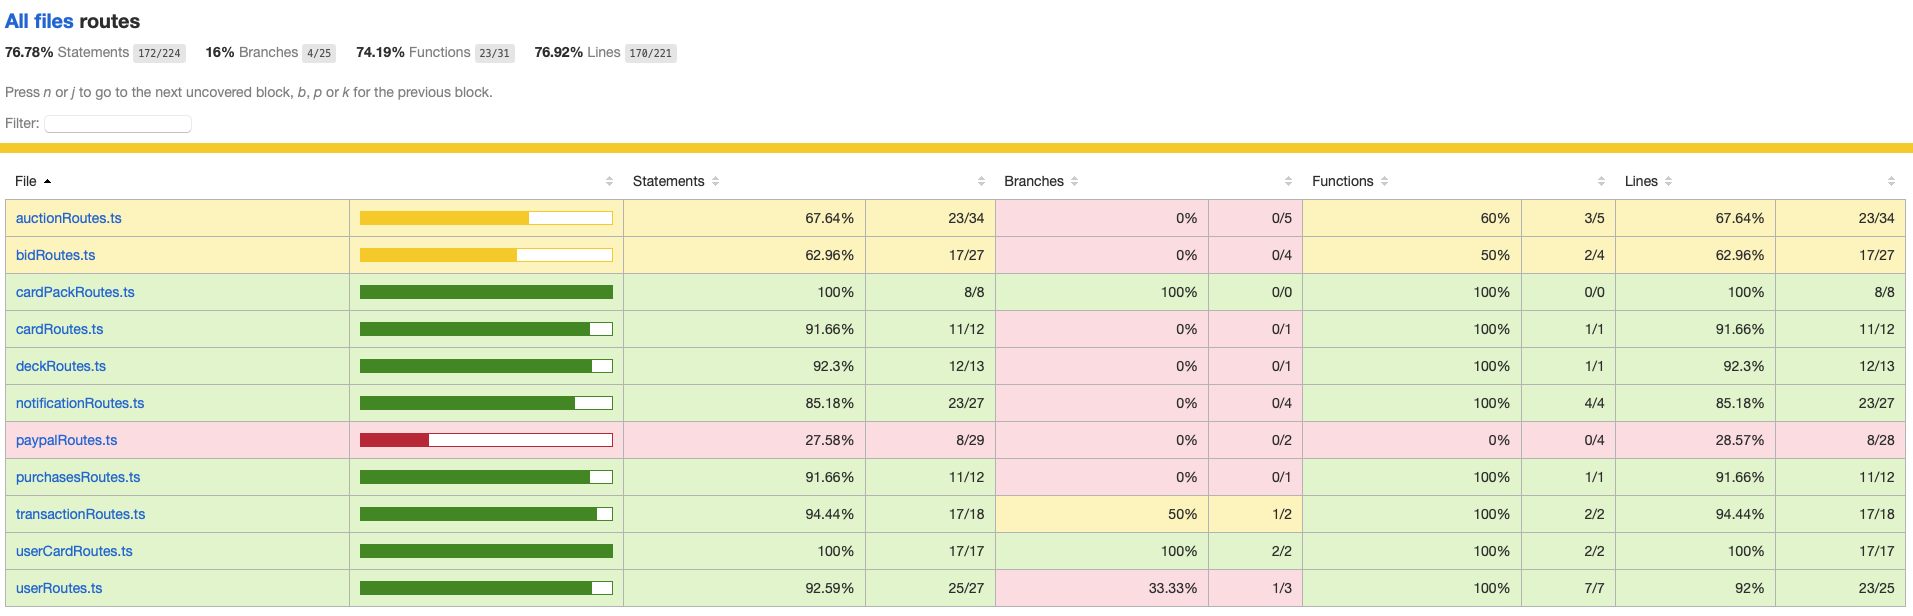
\includegraphics[width=0.8\linewidth]{figures/6-Analisis/6-Pruebas/6_8-Coverage-Restapi.png}
    \caption{Cobertura de Código del Subsistema restapi}
    \label{fig:6_8_Cobertura-Code-Restapi}
\end{figure}

A continuación, se detallan las pruebas unitarias realizadas en el subsistema \textbf{restapi}, con su descripición y resultado esperado.
Cabe destacar que para la ejecución de todas las pruebas, salvo para \textit{POST /api/users/login} y \textit{POST /api/users/signup}, se ha utilizado un token de autenticación válido, 
es decir, se ha iniciado sesión previamente con un usuario existente.
%-------------------TABLA PRUEBAS UNITARIAS RESTAPI-------------------

%-------------------TESTS DE AUCTIONROUTER-------------------
\begin{longtable}{
    >{\columncolor{lightgreen!20}}p{4cm}
    p{6cm}
    p{4cm}
    }
    \caption{Tests de auctionRouter} \label{table:test_auctionRouter} \\
    \toprule
    \rowcolor{darkgreen!50}
    \multicolumn{3}{|c|}{\textbf{Tests de auctionRouter}}\\
    \midrule
    \rowcolor{darkgreen!30}
    \textbf{Ruta a probar} & \multicolumn{1}{>{\columncolor{darkgreen!50}\centering\arraybackslash}p{6cm}}{\textbf{Descripción}} & \multicolumn{1}{>{\columncolor{darkgreen!50}\centering\arraybackslash}p{4cm}}{\textbf{Resultado esperado}} \\
    \endfirsthead
    
    \multicolumn{3}{c}%
    {{ \tablename\ \thetable{} Tests de auctionRouter -- continuación de la página anterior}} \\
    \toprule
    \rowcolor{darkgreen!50}
    \multicolumn{3}{|c|}{\textbf{Tests de auctionRouter}}\\
    \midrule
    \rowcolor{darkgreen!30}
    \textbf{Ruta a probar} & \multicolumn{1}{>{\columncolor{darkgreen!50}\centering\arraybackslash}p{6cm}}{\textbf{Descripción}} & \multicolumn{1}{>{\columncolor{darkgreen!50}\centering\arraybackslash}p{4cm}}{\textbf{Resultado esperado}} \\
    \midrule
    \endhead
    
    \midrule
    \multicolumn{3}{r}{{Continúa en la siguiente página...}} \\ 
    \endfoot
    
    \bottomrule
    \endlastfoot
    
    \midrule
    \textbf{GET /api/auctions} & Devuelve todas las subastas. & 200, la respuesta contiene una lista de subastas. \\
    \midrule
    \textbf{GET /api/auctions/a/:id} & Devuelve una subasta específica. & 200, la respuesta contiene los datos de la subasta. \\
    \midrule
    \textbf{GET /api/auctions/a/:id (no existe)} & Devuelve 404 si el ID de la subasta no se encuentra. & 404, la respuesta indica que la subasta no se encuentra. \\
    \midrule
    \textbf{GET /api/auctions/active/:username} & Devuelve todas las subastas activas para un nombre de usuario válido. & 200, la respuesta contiene una lista de subastas activas. \\
    \midrule
    \textbf{GET /api/auctions/active/u/:username} & Devuelve todas las subastas activas para un usuario. & 200, la respuesta contiene una lista de subastas activas. \\
    \end{longtable}

%-------------------TESTS DE BIDROUTER-------------------
\begin{longtable}{
    >{\columncolor{lightgreen!20}}p{4cm}
    p{6cm}
    p{4cm}
    }
    \caption{Tests de bidRouter} \label{table:test_bidRouter} \\
    \toprule
    \rowcolor{darkgreen!50}
    \multicolumn{3}{|c|}{\textbf{Tests de bidRouter}}\\
    \midrule
    \rowcolor{darkgreen!30}
    \textbf{Ruta a probar} & \multicolumn{1}{>{\columncolor{darkgreen!50}\centering\arraybackslash}p{6cm}}{\textbf{Descripción}} & \multicolumn{1}{>{\columncolor{darkgreen!50}\centering\arraybackslash}p{4cm}}{\textbf{Resultado esperado}} \\
    \endfirsthead
    
    \multicolumn{3}{c}%
    {{ \tablename\ \thetable{} Tests de bidRouter -- continuación de la página anterior}} \\
    \toprule
    \rowcolor{darkgreen!50}
    \multicolumn{3}{|c|}{\textbf{Tests de bidRouter}}\\
    \midrule
    \rowcolor{darkgreen!30}
    \textbf{Ruta a probar} & \multicolumn{1}{>{\columncolor{darkgreen!50}\centering\arraybackslash}p{6cm}}{\textbf{Descripción}} & \multicolumn{1}{>{\columncolor{darkgreen!50}\centering\arraybackslash}p{4cm}}{\textbf{Resultado esperado}} \\
    \midrule
    \endhead
    
    \midrule
    \multicolumn{3}{r}{{Continúa en la siguiente página...}} \\ 
    \endfoot
    
    \bottomrule
    \endlastfoot
    
    \midrule
    \textbf{GET /api/bids/b/:id} & Devuelve una oferta específica. & 200, la respuesta contiene los datos de la oferta. \\
    \midrule
    \textbf{GET /api/bids/b/:id (no existe)} & Devuelve 404 si el ID de la oferta no se encuentra. & 404, la respuesta indica que la oferta no se encuentra. \\
    \midrule
    \textbf{GET /api/bids/active/u/:username} & Devuelve todas las ofertas activas para un nombre de usuario válido. & 200, la respuesta contiene una lista de ofertas activas. \\
    \end{longtable}

%-------------------TESTS DE CARDPACKROUTER-------------------
\begin{longtable}{
    >{\columncolor{lightgreen!20}}p{4cm}
    p{6cm}
    p{4cm}
    }
    \caption{Tests de cardPackRouter} \label{table:test_cardPackRouter} \\
    \toprule
    \rowcolor{darkgreen!50}
    \multicolumn{3}{|c|}{\textbf{Tests de cardPackRouter}}\\
    \midrule
    \rowcolor{darkgreen!30}
    \textbf{Ruta a probar} & \multicolumn{1}{>{\columncolor{darkgreen!50}\centering\arraybackslash}p{6cm}}{\textbf{Descripción}} & \multicolumn{1}{>{\columncolor{darkgreen!50}\centering\arraybackslash}p{4cm}}{\textbf{Resultado esperado}} \\
    \endfirsthead
    
    \multicolumn{3}{c}%
    {{ \tablename\ \thetable{} Tests de cardPackRouter -- continuación de la página anterior}} \\
    \toprule
    \rowcolor{darkgreen!50}
    \multicolumn{3}{|c|}{\textbf{Tests de cardPackRouter}}\\
    \midrule
    \rowcolor{darkgreen!30}
    \textbf{Ruta a probar} & \multicolumn{1}{>{\columncolor{darkgreen!50}\centering\arraybackslash}p{6cm}}{\textbf{Descripción}} & \multicolumn{1}{>{\columncolor{darkgreen!50}\centering\arraybackslash}p{4cm}}{\textbf{Resultado esperado}} \\
    \midrule
    \endhead
    
    \midrule
    \multicolumn{3}{r}{{Continúa en la siguiente página...}} \\ 
    \endfoot
    
    \bottomrule
    \endlastfoot
    
    \midrule
    \textbf{GET /api/cardpacks} & Devuelve todos los paquetes de cartas disponibles. & 200, la respuesta contiene una lista de paquetes de cartas filtrados por disponibilidad. \\
    \end{longtable}

%-------------------TESTS DE CARDROUTER-------------------
\begin{longtable}{
    >{\columncolor{lightgreen!20}}p{4cm}
    p{6cm}
    p{4cm}
    }
    \caption{Tests de cardRouter} \label{table:test_cardRouter} \\
    \toprule
    \rowcolor{darkgreen!50}
    \multicolumn{3}{|c|}{\textbf{Tests de cardRouter}}\\
    \midrule
    \rowcolor{darkgreen!30}
    \textbf{Ruta a probar} & \multicolumn{1}{>{\columncolor{darkgreen!50}\centering\arraybackslash}p{6cm}}{\textbf{Descripción}} & \multicolumn{1}{>{\columncolor{darkgreen!50}\centering\arraybackslash}p{4cm}}{\textbf{Resultado esperado}} \\
    \endfirsthead
    
    \multicolumn{3}{c}%
    {{ \tablename\ \thetable{} Tests de cardRouter -- continuación de la página anterior}} \\
    \toprule
    \rowcolor{darkgreen!50}
    \multicolumn{3}{|c|}{\textbf{Tests de cardRouter}}\\
    \midrule
    \rowcolor{darkgreen!30}
    \textbf{Ruta a probar} & \multicolumn{1}{>{\columncolor{darkgreen!50}\centering\arraybackslash}p{6cm}}{\textbf{Descripción}} & \multicolumn{1}{>{\columncolor{darkgreen!50}\centering\arraybackslash}p{4cm}}{\textbf{Resultado esperado}} \\
    \midrule
    \endhead
    
    \midrule
    \multicolumn{3}{r}{{Continúa en la siguiente página...}} \\ 
    \endfoot
    
    \bottomrule
    \endlastfoot
    
    \midrule
    \textbf{GET /api/cards/:cardId} & Devuelve una carta por su ID. & 200, la respuesta contiene los datos de la carta, incluyendo el nombre 'bulbasaur'. \\
    \midrule
    \textbf{GET /api/cards/:cardId (no existe)} & Devuelve 404 si la carta no se encuentra. & 404, la respuesta contiene el mensaje 'Carta no encontrada.'. \\
    \midrule
    \textbf{GET /api/cards/:cardId (error)} & Maneja errores de forma adecuada. & 500, la respuesta contiene el mensaje 'Se ha producido un error al obtener la carta.'. \\
    \end{longtable}



%-------------------TESTS DE DECKROUTER-------------------

\begin{longtable}{
    >{\columncolor{lightgreen!20}}p{4cm}
    p{6cm}
    p{4cm}
    }
    \caption{Tests de deckRouter} \label{table:test_deckRouter} \\
    \toprule
    \rowcolor{darkgreen!50}
    \multicolumn{3}{|c|}{\textbf{Tests de deckRouter}}\\
    \midrule
    \rowcolor{darkgreen!30}
    \textbf{Ruta a probar} & \multicolumn{1}{>{\columncolor{darkgreen!50}\centering\arraybackslash}p{6cm}}{\textbf{Descripción}} & \multicolumn{1}{>{\columncolor{darkgreen!50}\centering\arraybackslash}p{4cm}}{\textbf{Resultado esperado}} \\
    \endfirsthead
    
    \multicolumn{3}{c}%
    {{ \tablename\ \thetable{} Tests de deckRouter -- continuación de la página anterior}} \\
    \toprule
    \rowcolor{darkgreen!50}
    \multicolumn{3}{|c|}{\textbf{Tests de deckRouter}}\\
    \midrule
    \rowcolor{darkgreen!30}
    \textbf{Ruta a probar} & \multicolumn{1}{>{\columncolor{darkgreen!50}\centering\arraybackslash}p{6cm}}{\textbf{Descripción}} & \multicolumn{1}{>{\columncolor{darkgreen!50}\centering\arraybackslash}p{4cm}}{\textbf{Resultado esperado}} \\
    \midrule
    \endhead
    
    \midrule
    \multicolumn{3}{r}{{Continúa en la siguiente página...}} \\ 
    \endfoot
    
    \bottomrule
    \endlastfoot
    
    \midrule
    \textbf{GET /api/decks} & Devuelve todos los mazos de cartas. & 200, la respuesta contiene una lista de mazos de cartas. \\
    \midrule
    \textbf{GET /api/decks/:deckid} & Devuelve un mazo de cartas por su ID. & 200, la respuesta contiene los datos del mazo de cartas, incluyendo 'deckId', 'name', 'type', y 'publicationDate'. \\
    \midrule
    \textbf{GET /api/decks (error)} & Maneja errores de forma adecuada al obtener todos los mazos de cartas. & 500, la respuesta contiene el mensaje 'Se ha producido un error al obtener los mazos de cartas.'. \\
    \midrule
    \textbf{GET /api/decks/:deckid (no existe)} & Devuelve 404 si el mazo de cartas no se encuentra. & 404, la respuesta contiene el mensaje 'Mazo de cartas no encontrado.'. \\
    \midrule
    \textbf{GET /api/decks/:deckid (error)} & Maneja errores de forma adecuada al obtener un mazo de cartas por su ID. & 500, la respuesta contiene el mensaje 'Se ha producido un error al obtener el mazo de cartas.'. \\
    \end{longtable}


%-------------------TESTS DE NOTIFICATIONROUTER-------------------
\begin{longtable}{
    >{\columncolor{lightgreen!20}}p{4cm}
    p{6cm}
    p{4cm}
    }
    \caption{Tests de notificationRouter} \label{table:test_notificationRouter} \\
    \toprule
    \rowcolor{darkgreen!50}
    \multicolumn{3}{|c|}{\textbf{Tests de notificationRouter}}\\
    \midrule
    \rowcolor{darkgreen!30}
    \textbf{Ruta a probar} & \multicolumn{1}{>{\columncolor{darkgreen!50}\centering\arraybackslash}p{6cm}}{\textbf{Descripción}} & \multicolumn{1}{>{\columncolor{darkgreen!50}\centering\arraybackslash}p{4cm}}{\textbf{Resultado esperado}} \\
    \endfirsthead
    
    \multicolumn{3}{c}%
    {{ \tablename\ \thetable{} Tests de notificationRouter -- continuación de la página anterior}} \\
    \toprule
    \rowcolor{darkgreen!50}
    \multicolumn{3}{|c|}{\textbf{Tests de notificationRouter}}\\
    \midrule
    \rowcolor{darkgreen!30}
    \textbf{Ruta a probar} & \multicolumn{1}{>{\columncolor{darkgreen!50}\centering\arraybackslash}p{6cm}}{\textbf{Descripción}} & \multicolumn{1}{>{\columncolor{darkgreen!50}\centering\arraybackslash}p{4cm}}{\textbf{Resultado esperado}} \\
    \midrule
    \endhead
    
    \midrule
    \multicolumn{3}{r}{{Continúa en la siguiente página...}} \\ 
    \endfoot
    
    \bottomrule
    \endlastfoot
    
    \midrule
    \textbf{GET /api/notifications/:username} & Devuelve todas las notificaciones para un nombre de usuario válido. & 200, la respuesta contiene una lista de notificaciones. \\
    \midrule
    \textbf{GET /api/notifications/unread/:username} & Devuelve todas las notificaciones no leídas para un nombre de usuario válido. & 200, la respuesta contiene una lista de notificaciones no leídas. \\
    \midrule
    \textbf{PATCH /api/notifications/notification/:notificationId/read} & Marca una notificación como leída. & 200, la respuesta indica éxito. \\
    \midrule
    \textbf{PATCH /api/notifications/read/:username} & Marca todas las notificaciones de un usuario como leídas. & 200, la respuesta indica éxito. \\
    \end{longtable}


%-------------------TESTS DE PURCHASESROUTER-------------------
\begin{longtable}{
    >{\columncolor{lightgreen!20}}p{4cm}
    p{6cm}
    p{4cm}
    }
    \caption{Tests de purchasesRouter} \label{table:test_purchasesRouter} \\
    \toprule
    \rowcolor{darkgreen!50}
    \multicolumn{3}{|c|}{\textbf{Tests de purchasesRouter}}\\
    \midrule
    \rowcolor{darkgreen!30}
    \textbf{Ruta a probar} & \multicolumn{1}{>{\columncolor{darkgreen!50}\centering\arraybackslash}p{6cm}}{\textbf{Descripción}} & \multicolumn{1}{>{\columncolor{darkgreen!50}\centering\arraybackslash}p{4cm}}{\textbf{Resultado esperado}} \\
    \endfirsthead
    
    \multicolumn{3}{c}%
    {{ \tablename\ \thetable{} Tests de purchasesRouter -- continuación de la página anterior}} \\
    \toprule
    \rowcolor{darkgreen!50}
    \multicolumn{3}{|c|}{\textbf{Tests de purchasesRouter}}\\
    \midrule
    \rowcolor{darkgreen!30}
    \textbf{Ruta a probar} & \multicolumn{1}{>{\columncolor{darkgreen!50}\centering\arraybackslash}p{6cm}}{\textbf{Descripción}} & \multicolumn{1}{>{\columncolor{darkgreen!50}\centering\arraybackslash}p{4cm}}{\textbf{Resultado esperado}} \\
    \midrule
    \endhead
    
    \midrule
    \multicolumn{3}{r}{{Continúa en la siguiente página...}} \\ 
    \endfoot
    
    \bottomrule
    \endlastfoot
    
    \midrule
    \textbf{POST /api/purchases/cardpack} & Compra un paquete de cartas exitosamente, disminuyendo la cantidad disponible del paquete y el saldo del usuario, creando cartas de usuario y transacciones. & 200, la respuesta indica éxito y las verificaciones post-compra son correctas. \\
    \midrule
    \textbf{POST /api/purchases/cardpack (usuario no existe)} & Maneja errores cuando el usuario no existe. & 500, la respuesta contiene el mensaje 'El usuario no existe.'. \\
    \midrule
    \textbf{POST /api/purchases/cardpack (saldo insuficiente)} & Maneja errores cuando el usuario no tiene suficiente saldo. & 500, la respuesta indica un error de saldo insuficiente. \\
    \midrule
    \textbf{POST /api/purchases/cardpack (paquete no existe)} & Maneja errores cuando el paquete de cartas no existe. & 500, la respuesta indica que el paquete de cartas no se encuentra. \\
    \midrule
    \textbf{POST /api/purchases/cardpack (paquete no disponible)} & Maneja errores cuando el paquete de cartas no está disponible. & 500, la respuesta indica que el paquete de cartas no está disponible. \\
    \end{longtable}



%-------------------TESTS DE TRANSACTIONROUTER-------------------
\begin{longtable}{
    >{\columncolor{lightgreen!20}}p{4cm}
    p{6cm}
    p{4cm}
    }
    \caption{Tests de transactionRouter} \label{table:descripcion_transactionRouter} \\
    \toprule
    \rowcolor{darkgreen!50}
    \multicolumn{3}{|c|}{\textbf{Tests de transactionRouter}}\\
    \midrule
    \rowcolor{darkgreen!30}
    \textbf{Ruta a probar} & \multicolumn{1}{>{\columncolor{darkgreen!50}\centering\arraybackslash}p{6cm}}{\textbf{Descripción}} & \multicolumn{1}{>{\columncolor{darkgreen!50}\centering\arraybackslash}p{4cm}}{\textbf{Resultado esperado}} \\
    \endfirsthead
    
    \multicolumn{3}{c}%
    {{ \tablename\ \thetable{} Tests de transactionRouter -- continuación de la página anterior}} \\
    \toprule
    \rowcolor{darkgreen!50}
    \multicolumn{3}{|c|}{\textbf{Tests de transactionRouter}}\\
    \midrule
    \rowcolor{darkgreen!30}
    \textbf{Ruta a probar} & \multicolumn{1}{>{\columncolor{darkgreen!50}\centering\arraybackslash}p{6cm}}{\textbf{Descripción}} & \multicolumn{1}{>{\columncolor{darkgreen!50}\centering\arraybackslash}p{4cm}}{\textbf{Resultado esperado}} \\
    \midrule
    \endhead
    
    \midrule
    \multicolumn{3}{r}{{Continúa en la siguiente página...}} \\ 
    \endfoot
    
    \bottomrule
    \endlastfoot
    
    \midrule
    \textbf{GET /api/transactions} & Devuelve todas las transacciones. & 200, la respuesta contiene una lista de transacciones. \\
    \midrule
    \textbf{GET /api/transactions/u/:username} & Devuelve las transacciones para un nombre de usuario válido. & 200, la respuesta contiene una lista de transacciones para el usuario. \\
    \midrule
    \textbf{GET /api/transactions/c/:userCardId} & Devuelve las transacciones para un ID de carta de usuario válido. & 200, la respuesta contiene una lista de transacciones para la carta de usuario. \\
    \midrule
    \textbf{GET /api/transactions (no admin)} & Devuelve 403 si el usuario no es administrador. & 403, la respuesta contiene el mensaje 'Acceso denegado. Se requiere rol de administrador.'. \\
    \midrule
    \textbf{GET /api/transactions/u/:username (username inválido)} & Devuelve 400 para un nombre de usuario inválido. & 400, la respuesta contiene errores de validación para el nombre de usuario. \\
    \end{longtable}



%-------------------TESTS DE USERCARDROUTER-------------------
\begin{longtable}{
    >{\columncolor{lightgreen!20}}p{4cm}
    p{6cm}
    p{4cm}
    }
    \caption{Tests de userCardRouter} \label{table:test_userCardRouter} \\
    \toprule
    \rowcolor{darkgreen!50}
    \multicolumn{3}{|c|}{\textbf{Tests de userCardRouter}}\\
    \midrule
    \rowcolor{darkgreen!30}
    \textbf{Ruta a probar} & \multicolumn{1}{>{\columncolor{darkgreen!50}\centering\arraybackslash}p{6cm}}{\textbf{Descripción}} & \multicolumn{1}{>{\columncolor{darkgreen!50}\centering\arraybackslash}p{4cm}}{\textbf{Resultado esperado}} \\
    \endfirsthead
    
    \multicolumn{3}{c}%
    {{ \tablename\ \thetable{} Tests de userCardRouter -- continuación de la página anterior}} \\
    \toprule
    \rowcolor{darkgreen!50}
    \multicolumn{3}{|c|}{\textbf{Tests de userCardRouter}}\\
    \midrule
    \rowcolor{darkgreen!30}
    \textbf{Ruta a probar} & \multicolumn{1}{>{\columncolor{darkgreen!50}\centering\arraybackslash}p{6cm}}{\textbf{Descripción}} & \multicolumn{1}{>{\columncolor{darkgreen!50}\centering\arraybackslash}p{4cm}}{\textbf{Resultado esperado}} \\
    \midrule
    \endhead
    
    \midrule
    \multicolumn{3}{r}{{Continúa en la siguiente página...}} \\ 
    \endfoot
    
    \bottomrule
    \endlastfoot
    
    \midrule
    \textbf{GET /api/usercards/u/:username} & Devuelve las tarjetas de usuario para un nombre de usuario válido. & 200, la respuesta contiene un arreglo de tarjetas de usuario. \\
    \midrule
    \textbf{GET /api/usercards/:id} & Devuelve una tarjeta de usuario específica. & 200, la respuesta contiene la tarjeta de usuario con el campo 'legibleCardId'. \\
    \midrule
    \textbf{GET /api/usercards/:id (no existe)} & Devuelve 404 si la tarjeta de usuario no se encuentra. & 404, la respuesta indica que la tarjeta de usuario no se encuentra. \\
    \midrule
    \textbf{GET /api/usercards/:id (ID inválido)} & Devuelve 400 para un ID de tarjeta de usuario inválido. & 400, la respuesta indica un error. \\
    \midrule
    \textbf{GET /api/usercards/u/:username (nombre de usuario muy largo)} & Devuelve 400 si el nombre de usuario es demasiado largo. & 400, la respuesta indica un error con un mensaje sobre la longitud del nombre de usuario. \\
    \end{longtable}

%-------------------TESTS DE USERROUTER-------------------
\begin{longtable}{
    >{\columncolor{lightgreen!20}}p{4cm}
    p{6cm}
    p{4cm}
    }
    \caption{Tests de userRouter} \label{table:test_userRouter} \\
    \toprule
    \rowcolor{darkgreen!50}
    \multicolumn{3}{|c|}{\textbf{Tests de userRouter}}\\
    \midrule
    \rowcolor{darkgreen!30}
    \textbf{Ruta a probar} & \multicolumn{1}{>{\columncolor{darkgreen!50}\centering\arraybackslash}p{6cm}}{\textbf{Descripción}} & \multicolumn{1}{>{\columncolor{darkgreen!50}\centering\arraybackslash}p{4cm}}{\textbf{Resultado esperado}} \\
    \endfirsthead
    
    \multicolumn{3}{c}%
    {{ \tablename\ \thetable{} Tests de userRouter -- continuación de la página anterior}} \\
    \toprule
    \rowcolor{darkgreen!50}
    \multicolumn{3}{|c|}{\textbf{Tests de userRouter}}\\
    \midrule
    \rowcolor{darkgreen!30}
    \textbf{Ruta a probar} & \multicolumn{1}{>{\columncolor{darkgreen!50}\centering\arraybackslash}p{6cm}}{\textbf{Descripción}} & \multicolumn{1}{>{\columncolor{darkgreen!50}\centering\arraybackslash}p{4cm}}{\textbf{Resultado esperado}} \\
    \midrule
    \endhead
    
    \midrule
    \multicolumn{3}{r}{{Continúa en la siguiente página...}} \\ 
    \endfoot
    
    \bottomrule
    \endlastfoot
    
    \midrule
    \textbf{POST /api/users/login} & Inicia sesión un usuario existente con el nombre de usuario 'test' y la contraseña 'Password123-'. & 200, la respuesta contiene un token y datos del usuario. \\
    \midrule
    \textbf{POST /api/users/signup} & Crea un nuevo usuario con el nombre de usuario 'newuser' y la contraseña 'Password123-'. & 201, la respuesta contiene un mensaje de éxito y datos del nuevo usuario. \\
    \midrule
    \textbf{GET /api/users/:username} & Obtiene los detalles del usuario 'test' con un token válido. & 200, la respuesta contiene los datos del usuario. \\
    \midrule
    \textbf{PATCH /api/users/update/avatar} & Actualiza la imagen de perfil del usuario 'test' a 'avatar1.png'. & 200, la respuesta indica éxito. \\
    \midrule
    \textbf{PATCH /api/users/update/pass} & Actualiza la contraseña del usuario 'test' a 'NewPass1234-'. & 200, la respuesta indica éxito. \\
    \midrule
    \textbf{GET /api/users/:username (error handling)} & Devuelve 400 si el nombre de usuario es demasiado largo. & 400, la respuesta indica error. \\
    \midrule
    \textbf{GET /api/users/:username (sin token)} & Devuelve 401 si no se proporciona un token. & 401, la respuesta indica error. \\
    \midrule
    \textbf{GET /api/users/:username (usuario no encontrado)} & Devuelve 404 si el usuario no se encuentra. & 404, la respuesta contiene mensaje de usuario no encontrado. \\
    \midrule
    \textbf{GET /api/users/:username (error)} & Maneja errores de forma adecuada. & 500, la respuesta indica error interno. \\
    \midrule
    \textbf{POST /api/users/login (usuario no existe)} & Devuelve 401 si el usuario no existe. & 401, la respuesta indica error. \\
    \midrule
    \textbf{POST /api/users/login (contraseña incorrecta)} & Devuelve 401 si la contraseña es incorrecta. & 401, la respuesta indica error. \\
    \midrule
    \textbf{POST /api/users/login (error)} & Maneja errores de forma adecuada. & 500, la respuesta indica error interno. \\
    \midrule
    \textbf{POST /api/users/signup (usuario ya existe)} & Devuelve 400 si el nombre de usuario ya existe. & 400, la respuesta indica error. \\
    \midrule
    \textbf{POST /api/users/signup (datos incompletos)} & Devuelve 400 si falta el nombre de usuario, contraseña o fecha de nacimiento. & 400, la respuesta indica error. \\
    \midrule
    \textbf{POST /api/users/signup (error)} & Maneja errores de forma adecuada. & 500, la respuesta contiene mensaje de error y autenticación fallida. \\
    \end{longtable}




\subsubsubsection{Pruebas Unitarias. Webapp}
En el subsistema \textbf{webapp} se han realizado 5 pruebas unitarias automáticas, se han probado los componentes más importantes de la aplicación y todas han pasado con éxito.
El resto de componentes se han probado de forma manual y se ha comprobado que su comportamiento es el esperado.


\subsubsection{Pruebas de Integración}
Las pruebas de integración se han realizado con éxito, se han comprobado que los distintos componentes del sistema funcionan correctamente en conjunto.
Se han realizado pruebas de integración en el subsistema \textbf{webapp} con el framework jest-cucumber y Puppeteer.
Se han realizado 3 pruebas de integración automáticas, todas ellas han pasado con éxito.
Las pruebas que se han realizado son las siguientes:
\begin{itemize}
    \item \textbf{Prueba de Inicio de Sesión Exitoso}: Se ha comprobado que el inicio de sesión funciona correctamente. De esta forma, se ha comprobado que el usuario puede iniciar sesión con sus credenciales y acceder a la aplicación, 
    lo que significa que la conexión con el backend funciona correctamente y la integración de los componentes de la aplicación es correcta.
    \item \textbf{Prueba de Inicio de Sesión Fallido}: Se ha comprobado que el inicio de sesión falla cuando las credenciales son incorrectas. De esta forma, se ha comprobado que la aplicación responde correctamente a errores en el inicio de sesión.
     \item \textbf{Prueba de Registro de Usuario Fallido}: Se ha comprobado que el registro de usuario falla cuando los datos introducidos no son válidos. 
     Se verifica que la aplicación responde correctamente a errores en el registro de usuario y se resaltan los campos con errores.
\end{itemize}

El resto de pruebas de integración se han realizado de forma manual y se ha comprobado que el comportamiento de la aplicación es el esperado.

\subsubsection{Pruebas de Usabilidad}
Se ha creado un formulario de evaluación de usabilidad que se les ha proporcionado a los usuarios para que evalúen la interfaz de usuario.
Se han realizado pruebas de usabilidad con 3 usuarios reales, que han evaluado la interfaz de usuario y han proporcionado retroalimentación sobre su usabilidad.
Estos usuarios, que no han participado en el desarrollo de la aplicación, han tenido que completar una serie de tareas y responder a preguntas sobre la usabilidad de la aplicación.
Los usuarios tienen una experiencia variada en el uso de aplicaciones web y representan a los diferentes tipos de usuarios que utilizarán la aplicación.
Los datos de los usuarios son los siguientes:
\begin{itemize}
    \item \textbf{Usuario 1}: Hombre de 51 años, con poca experiencia en el uso de aplicaciones web. No ha utilizado aplicaciones similares anteriormente ni realizado compras en línea.
    \item \textbf{Usuario 2}: Mujer de 22 años, con mucha experiencia en el uso de aplicaciones web. Ha utilizado aplicaciones similares anteriormente y ha realizado compras en línea.
    \item \textbf{Usuario 3}: Mujer de 18 años, con experiencia en el uso de aplicaciones web. Ha utilizado aplicaciones similares anteriormente, pero no ha llegado a realizar compras en ellas.
\end{itemize}

\subsubsubsection{Cuestionario de usabilidad}
Se ha realizado un cuestionario de usabilidad con distintas preguntas para evaluar la calidad de la interfaz de usuario de la aplicación.
Estas preguntas pretenden evaluar la calidad del diseño de la interfaz, la facilidad de uso y la satisfacción del usuario.
Este cuestionario se ha proporcionado a los usuarios para que lo completen después de realizar las tareas asignadas.
En la tabla  \coloredUnderline{\hyperlink{table:cuestionario_usabilidad}{Tabla \ref*{table:cuestionario_usabilidad}. \nameref*{table:cuestionario_usabilidad}}} se muestra el cuestionario de usabilidad que se ha proporcionado a los usuarios.

\begin{longtable}{ \hypertarget{table:cuestionario_usabilidad}{}
    >{\columncolor{lightgreen!20}}p{4cm}
    >{\centering\arraybackslash}p{1.3cm}
    >{\centering\arraybackslash}p{1.3cm}
    >{\centering\arraybackslash}p{1.3cm}
    >{\centering\arraybackslash}p{1.3cm}
    >{\centering\arraybackslash}p{1.3cm}
    }
    \caption{Cuestionario de usabilidad de la aplicación} \label{table:cuestionario_usabilidad} \\
    \toprule
    \rowcolor{darkgreen!50}
    \textbf{Pregunta} & \multicolumn{4}{>{\columncolor{darkgreen!50}\centering\arraybackslash}p{1.3cm}}{\textbf{1}} & \multicolumn{1}{>{\columncolor{darkgreen!50}\centering\arraybackslash}p{1.3cm}}{\textbf{2}}  & \multicolumn{1}{>{\columncolor{darkgreen!50}\centering\arraybackslash}p{1.3cm}}{\textbf{3}}  & \multicolumn{1}{>{\columncolor{darkgreen!50}\centering\arraybackslash}p{1.3cm}}{\textbf{4}}  & \multicolumn{1}{>{\columncolor{darkgreen!50}\centering\arraybackslash}p{1.3cm}}{\textbf{5}} \\
    \endfirsthead
    
    \multicolumn{6}{c}%
    {{ \tablename\ \thetable{} Cuestionario de usabilidad de la aplicación -- continuación de la página anterior}} \\
    \toprule
    \rowcolor{darkgreen!50}
   \textbf{Pregunta} & \multicolumn{4}{>{\columncolor{darkgreen!50}\centering\arraybackslash}p{1.3cm}}{\textbf{1}} & \multicolumn{1}{>{\columncolor{darkgreen!50}\centering\arraybackslash}p{1.3cm}}{\textbf{2}}  & \multicolumn{1}{>{\columncolor{darkgreen!50}\centering\arraybackslash}p{1.3cm}}{\textbf{3}}  & \multicolumn{1}{>{\columncolor{darkgreen!50}\centering\arraybackslash}p{1.3cm}}{\textbf{4}}  & \multicolumn{1}{>{\columncolor{darkgreen!50}\centering\arraybackslash}p{1.3cm}}{\textbf{5}} \\
    
    \midrule
    \endhead
    
    \midrule
    \multicolumn{6}{r}{{Continúa en la siguiente página...}} \\ 
    \endfoot
    
    \bottomrule
    \endlastfoot
    
    \midrule
    \rowcolor{lightgray}
    \multicolumn{6}{|c|}{Calidad del Interfaz} \\
    \midrule
    El tipo y tamaño de letra es & & & & & \\
    \midrule
    Los iconos e imágenes usados son & & & & & \\
    \midrule
    Los colores empleados son & & & & & \\
    \midrule
    La organización de los elementos es & & & & & \\
    \midrule
    Las estructuras de las tablas son & & & & & \\
    \midrule
\end{longtable}
